\documentclass[SKL-MASTER.tex]{subfiles}
\begin{document}
	\Large
\section*{Calculating an ROC Curve in Python} 
\begin{itemize}
\item scikit-learn makes it easy to calculate ROC Curves. 
\item Firstly, we need a classification model to evaluate. 
\item For this example, we will make a synthetic dataset and then build a logistic regression model using scikit-learn.
\end{itemize}

{
	\Large
\begin{framed}
	\begin{verbatim}
from sklearn.datasets import make_classification
from sklearn.linear_model import LogisticRegression

# Make a Simulated Data Set
X, y = make_classification(n_samples=10000, 
         n_features=10, n_classes=2,
         n_informative=5)
         
# Split it into Testing and Training Sets         
Xtrain = X[:9000]
Xtest = X[9000:]
ytrain = y[:9000]
ytest = y[9000:]

# Train the Model
clf = LogisticRegression()
clf.fit(Xtrain, ytrain)


# Apply model to Testing Data
preds = clf.predict_proba(Xtest)[:,1]

\end{verbatim}
\end{framed}
}
%Now that we have our model we can calculate the ROC curve. Pretty easy--from scikit-learn import roc_curve, pass in the actual y values from our test set and the predicted probabilities for those same records.
%
%The results will yield your FPR and TPR. Pass those into a ggplot and BAM! You've got yourself a nice looking ROC curve.
\newpage
{
	\large
\begin{framed}
\begin{verbatim}
from sklearn import metrics
import pandas as pd
from ggplot import *


fpr, tpr, _ = metrics.roc_curve(ytest, preds)

## Create as DataFrame

df = pd.DataFrame(dict(fpr=fpr, tpr=tpr))

## ggplote takes pandas Data frames as arguments

ggplot(df, aes(x='fpr', y='tpr')) +
    geom_line() + geom_abline(linetype='dashed')

\end{verbatim}
\end{framed}
}
\begin{figure}[h!]
\centering
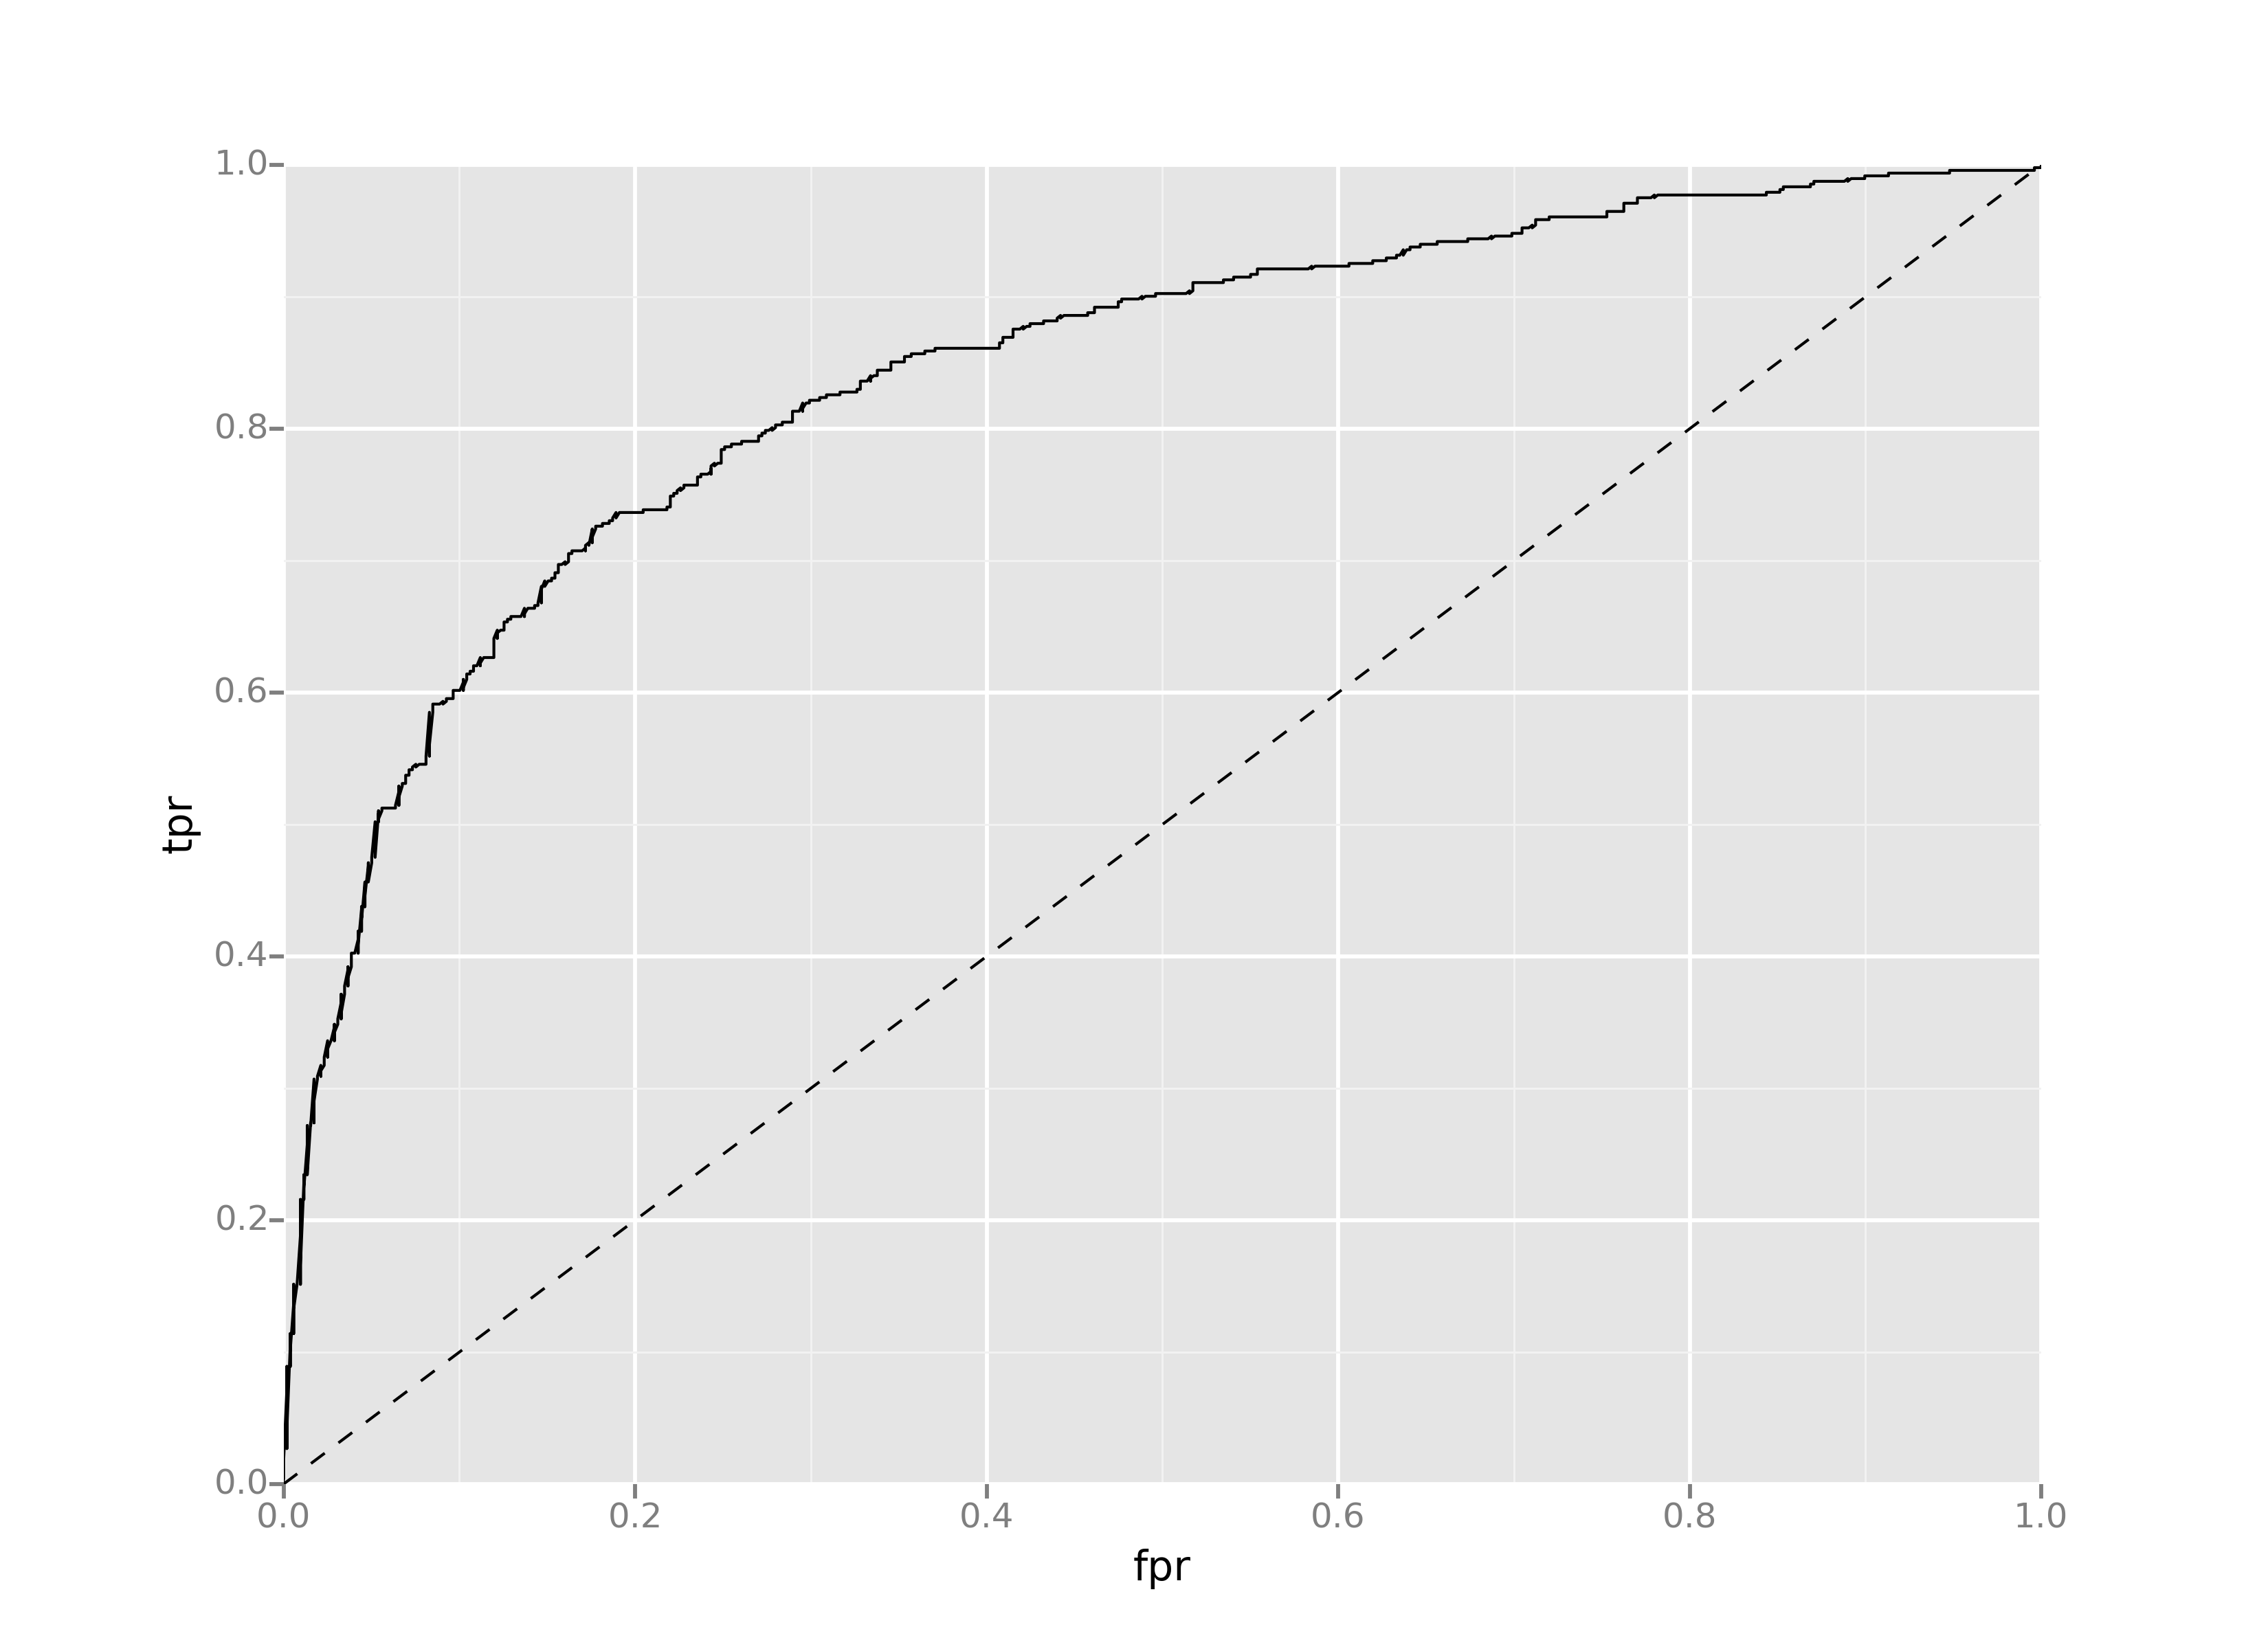
\includegraphics[width=0.99\linewidth]{images/roc-python}

\end{figure}

\newpage
Finally to calculate the AUC:
{
	\large
\begin{framed}
	\begin{verbatim}
auc = metrics.auc(fpr,tpr)

# Add this to the plot
#  - see the "ggtitle" option

ggplot(df, aes(x='fpr', ymin=0, ymax='tpr')) +
    geom_area(alpha=0.2) +
    geom_line(aes(y='tpr')) +
    ggtitle("ROC Curve w/ AUC=%s" % str(auc))
 \end{verbatim}
\end{framed}
}
The AUC is 0.900. 
\begin{figure}[h!]
\centering
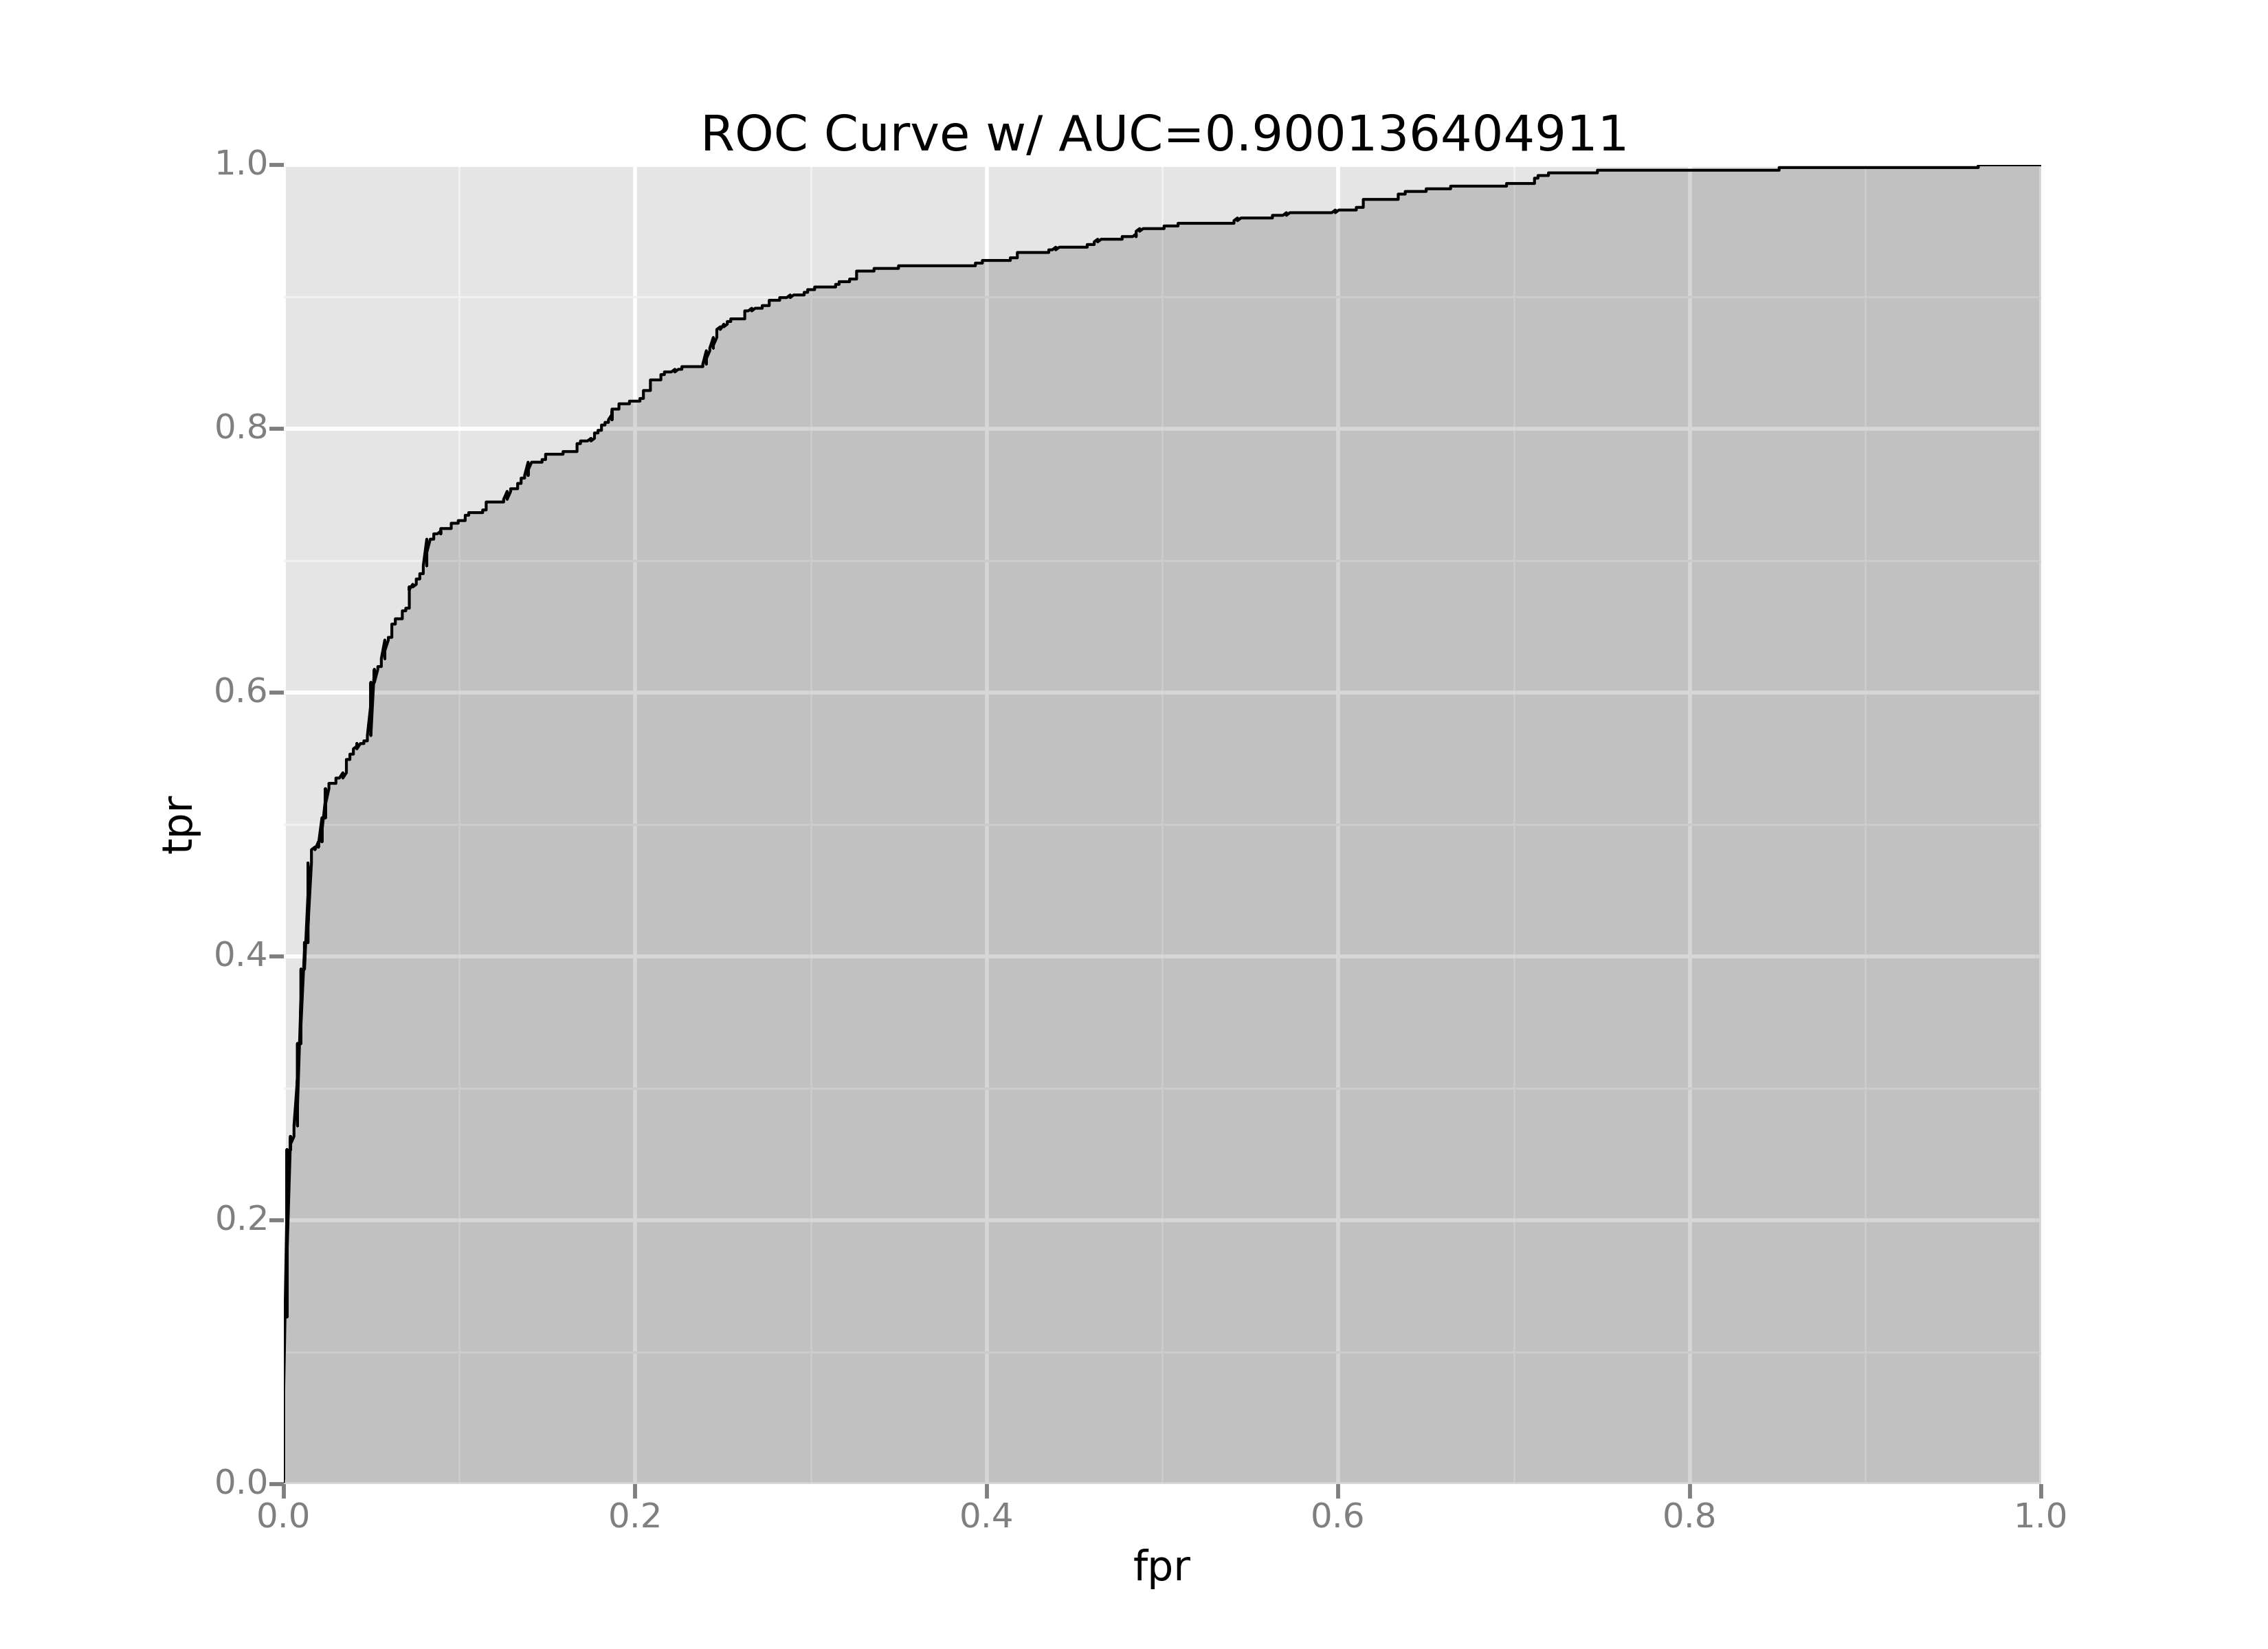
\includegraphics[width=0.99\linewidth]{images/roc-with-auc-python}

\end{figure}

% Recalling from earlier, AUC is bounded between 0 and 1, so this is pretty good.

\end{document}